\documentclass[11pt]{article}
\usepackage{latexsym}
\usepackage{amssymb,amsmath}
\usepackage[pdftex]{graphicx}
% \usepackage{qtree}

\topmargin = -.75in \textwidth=7in \textheight=9.3in
\oddsidemargin = -.3in \evensidemargin = -.3in

\begin{document}
\begin{center}
\large
CS181 Assignment 2
\end{center}
Joy Ming and Alisa Nguyen (25 February 2013)\\

\begin{enumerate}
\setcounter{enumi}{0}

\item Perceptron activation rule
	\begin{enumerate}
	\item Bright-or-dark is not able to be recognized by a perceptron. One possibility is to have the weights of all $n=9$ pixels be initialized to $1/n=1/9$. Then, multiplying the value if the pixel is on (1) or off (0) with the weights will give something greater than 0.75 if at least 75\% pixels are on and will give something less than 0.25 if at least 75\% pixels are off. However, this function of returning positive when the value is greater than 0.75 and less than 0.25 is piecewise and not differentiable. There cannot exist a perceptron that recognizes this feature because this feature is not linearly separable.
	% This perceptron would have the weights of all $n=9$ pixels to be initialzed to $1/n=1/9$. Then, multiplying the value if the pixel is on (1) or off (0) with the weights will give something greater than 0.75 if at least 75\% pixels are on and will give something less than 0.35 if at least 75\% pixels are off.
	\item Top-bright is able to be recognized by a perceptron. This perceptron would have $1/3$ weights for the top three pixels and $-1/6$ weights for the bottom pixels. If both have the same fraction of pixels on in both rows then the result should be 0. However, if the top has a larger fraction it would be positive and if the bottom has a larger fraction it would be negative. Therefore, simply checking to see if the result is greater than zero can tell if a larger fraction of pixels is on the top row than in the bottom two rows.
	\item It is not possible to present a perceptron that can check to see if a set of pixels that are on is connected because it is not possible to model when different points of data are correlated. Suppose for contradiction that there is a perceptron that could check to see if a set of pixels that are on is connected. Then for PROOF.
	\end{enumerate}
\item Four different possible learning algorithms
	\begin{enumerate}
	\item Decision trees are most effective when there are characteristics to split on with different values. However, it is difficult in this case to even determine which characteristics to split on, even if there were some way to implement continuous attributes. One possibility for splitting would be starting from a given pixel such as the top left pixel to see if its neighbors are activated or not. However, this would result in a lot of branches for each pixel and its neighbors. This could also be difficult to train and determine these splits.
	\item Boosted decision stumps are especially useful for making prediction based on the value of a single input feature over a specific threshold. Though these decision stumps can reach a higher level of accuracy after boosting, their level of simplicity that contrasts that of the complicated features of the decision trees is well adapted for the problem. One way to approach this would be to have a separate decision stump for each pixel. However, this would result in it being very difficult to figure out the linking of the different, separate pixels. Combatting this inability to consider connected features would be to track the presence of certain patterns. However, it would still be difficult to even put the frequency of these patterns together as well.
	\item Perceptrons are better than decision trees and decision stumps at learning about the set of data as opposed to individual pixels. This is because the perceptrons are looking at the sum of the different pixels. However, perceptrons do have some weaknesses, as evidenced by the previous problems. They are still limited only to linearly separable data and their decision boundaries have to be based on differentiable functions that will not be able to consider piecewise functions or connectedness. Therefore, though perceptrons are a step toward understanding, there have to be more layers to get a better grasp of the data. 
	\item Multi-layer feed-forward neural networks is what we implemented in the problem set, which speaks to its validity as a means of approaching the problem of digit recognition. This problem has as many as 196 pixels for a 14x14 image, as spoken about many times in discounting the other methods. The multi-layer feed-forward network can help with this in that it can take many different inputs. The problem of digit recognition also has 10 distinct output categories, which is well embodied by the various output nodes in the multi-layer feed forward neural networks. One drawback is that this needs a lot of previous knowledge. 
	\end{enumerate}
\item Implementing a neural network
\newline
\newline
5. We normalize the input values from [0, 255] to between 0 and 1 so we are able to better utilize the logistic sigmoid function.\\ 
\newline
6. Experiment with simple networks
\begin{enumerate}
\item We used a learning rate of 0.1 based on this DATA:
\item
$$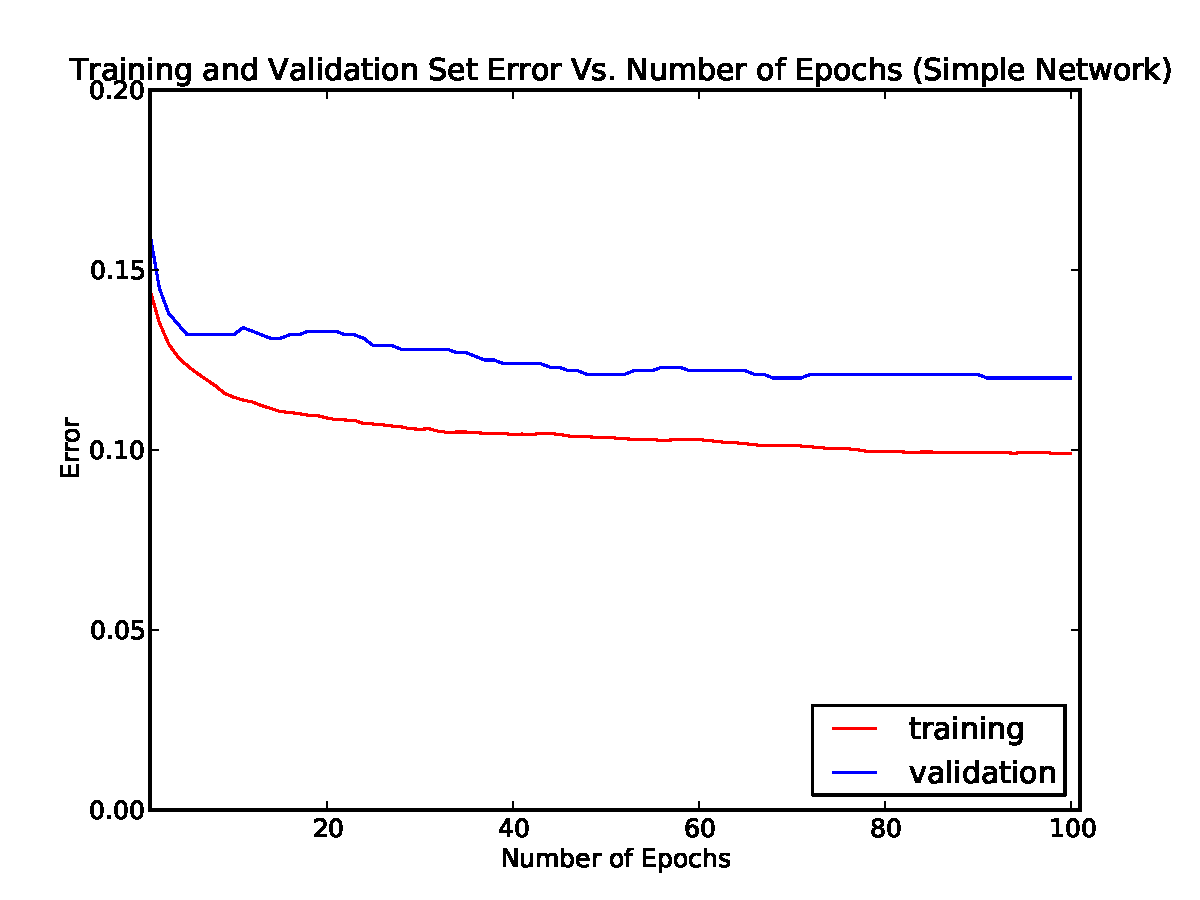
\includegraphics[width=150mm]{nguyen-ming-36b.pdf}$$ 
\begin{enumerate}
\item Yes/No we are/are not in danger of overfitting by training for too many epochs.
\item A good number of epochs to train for is
\\It is important that we use a validation set rather than the actual test set to tune the number of epochs because
\end{enumerate}
\item The training performance is
\\ The validation performance is
\\ The test performance is
\end{enumerate} 
7. Experiment with networks with a single hidden layer
\begin{enumerate}
\item We decided that we wanted to use a learning rate of 0.3 for both 15 and 30 fully connected units in the hidden layer based on DATA.
\item We determine when to stop training by checking the difference between the validation performance and the previous validation performance. If the difference is less than a given $\epsilon$, which in this case was 0.001, at least five times in a row, then stop the training.
\item $$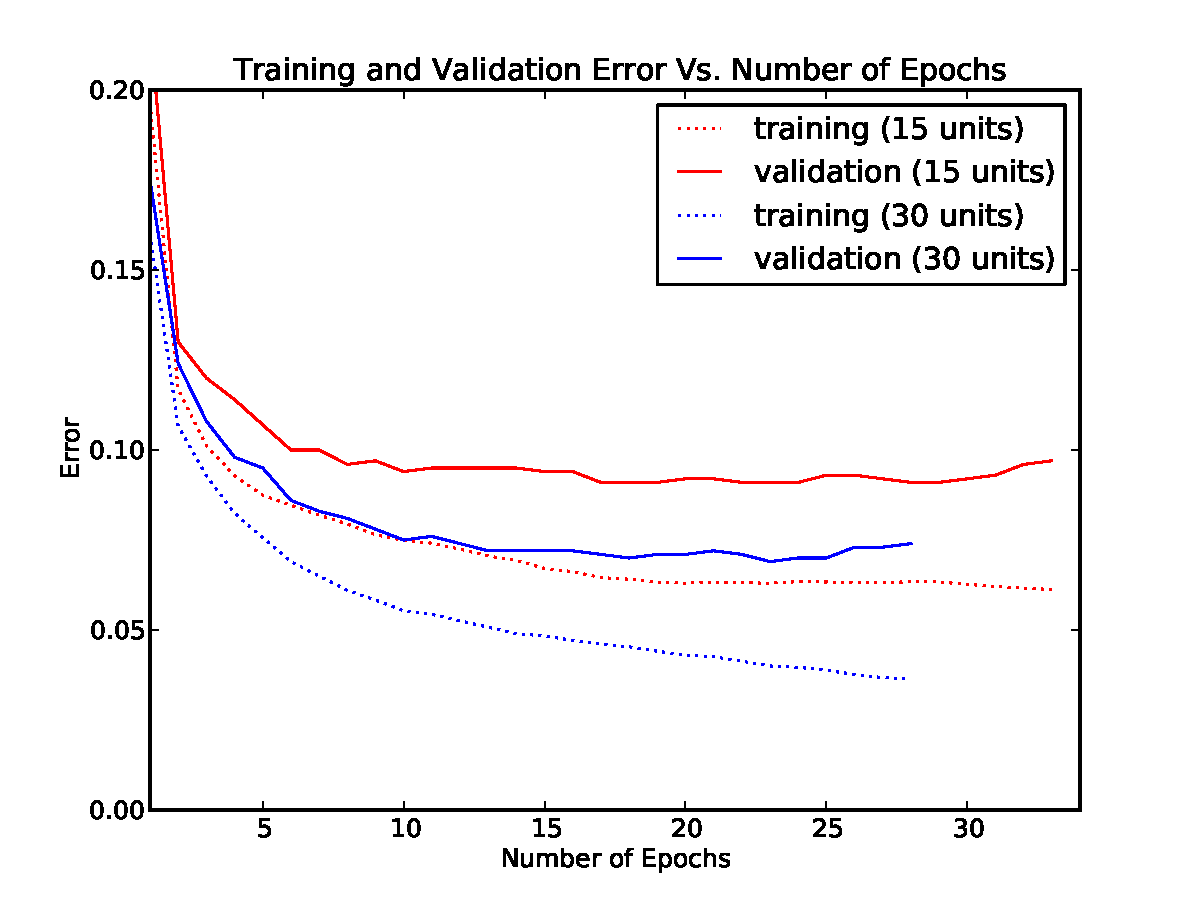
\includegraphics[width=150mm]{nguyen-ming-37c.pdf}$$
\item We used 33 epochs for 15 hidden units and 28 epochs for 30 hidden units.
\item Based on these experiements, we would use the network structure with 30 fully connected hidden units because both training set error and validation set error were lower for the 30 fully connected hidden units compared to the 15. By the 28th epoch round for the 30 hidden units, the training set error was 0.036 and the validation set error was 0.074, which is considerably less than the errors for 15 units by the 33rd round, which were 0.612 and 0.097 respectively.
\item The test set performance of the network with 30 hidden units for 28 epochs was \fbox{0.949}. This is higher than the test set performance of the network with 15 hidden units for 33 epochs, which was 0.939. This compares to the committee of perceptrons by FILLIN.
\end{enumerate}
8. CustomNetwork
\begin{enumerate}
\item We chose to implement more hidden layers to see how this impacts the performance of the neural networks. First we put in two hidden layers of 15 then we put in three hidden layers of 10. 
\item Our new network's test performances include:
\item It was surprising, at first that the performances were so drastically different. However, thinking more about the data, it seemed to make more sense 
\end{enumerate}
\item Changing error function
	\begin{enumerate}
	\item Error function $C$ is implementing the idea of regularization, or that the less complex solution, or one that has less dimensions or degrees, is more desirable others that might work. In the new error function, different values are added onto the original loss function that will increase the sum depending on the increased complexity or layers of the network. This will penalize the loss function by squared weight values, making it more crucial to create less complicated graphs to minimize the loss function. 
	\item Our weight update rule for the error function $C$ derived from gradient descent is:
	\end{enumerate}

\end{enumerate}
\end{document}